\begin{figure}[t]
    \centering
    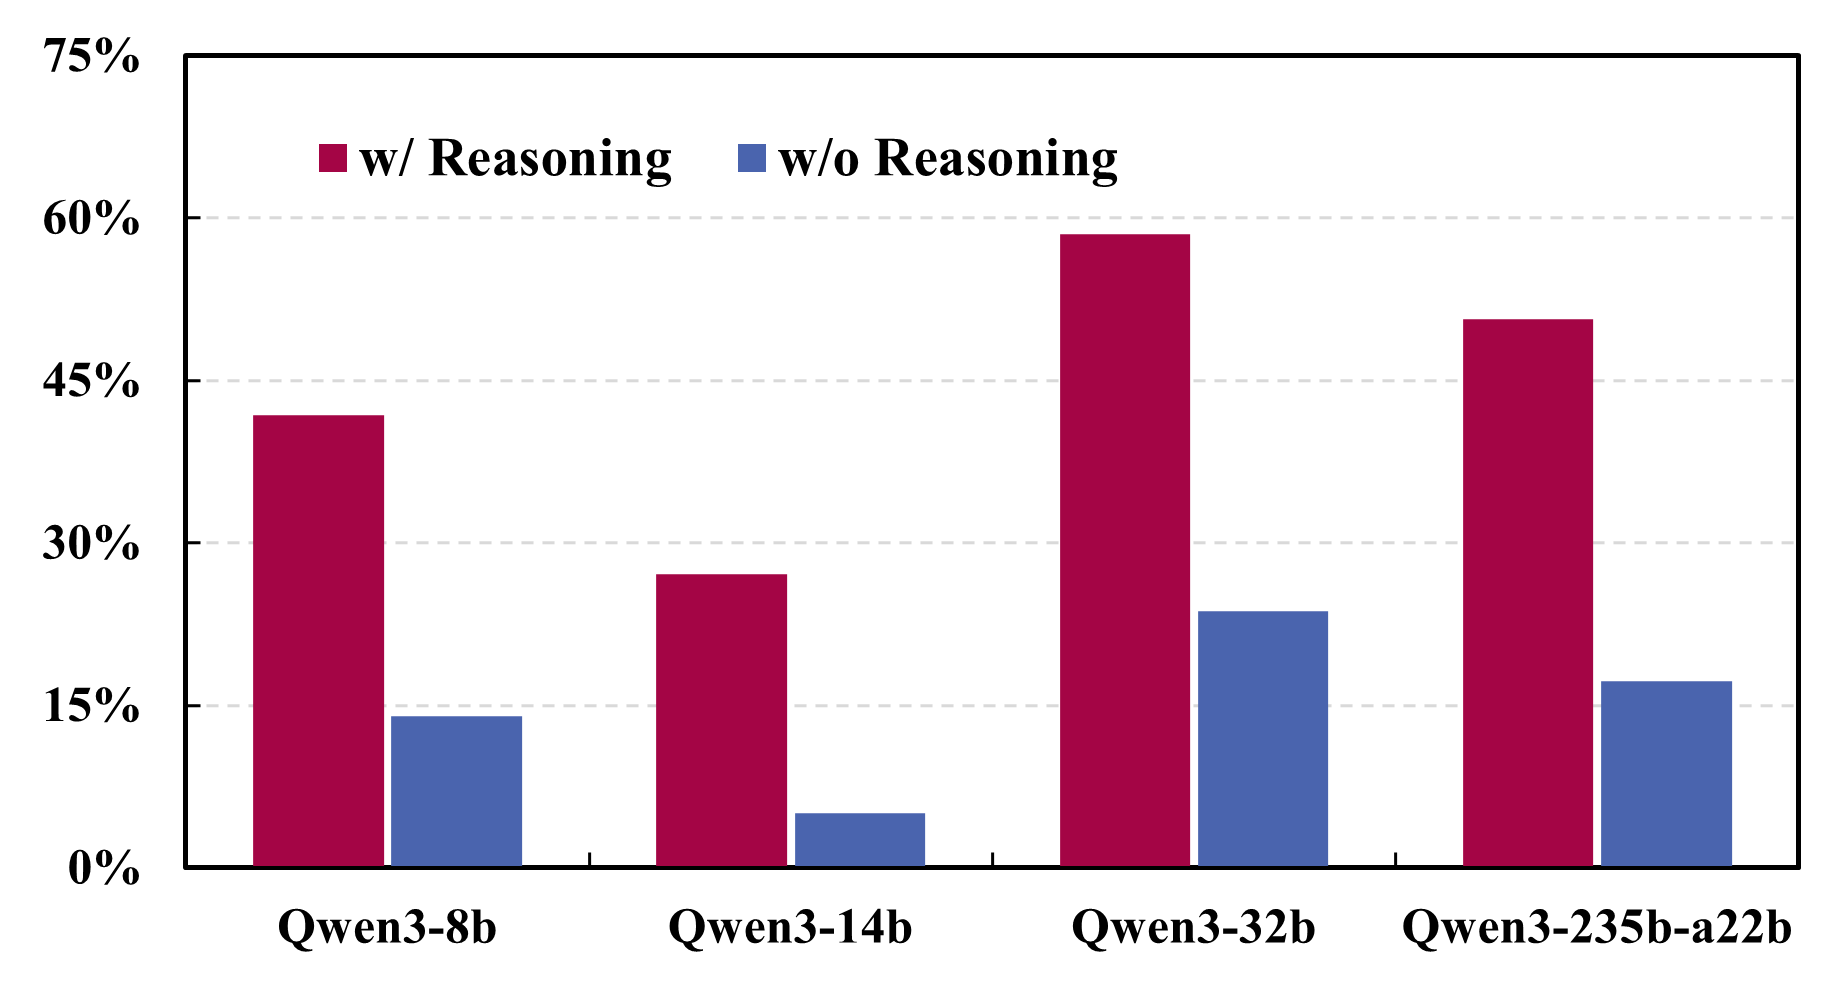
\includegraphics[width=.48\textwidth]{figs/model-cha.png}
    \caption{ASR of different scales and reasoning settings.}
    % 动态隐私需求可扩展性举例。s1阶段隐私任务是年龄分类，s2阶段隐私任务增加了性别分类，s3阶段继续增加种族分类。我们只修改UIE模块即可满足动态变化的隐私需求。
    \label{fig:reasoning-settings}
    % \vspace{-1em}
\end{figure}
\section{Experiments}
\subsection{Experiment Settings}

% \begin{table*}[h]

% \renewcommand{\arraystretch}{1.3}
% \centering

% \begin{tabular}{@{}lccccccccccccc@{}}

% \toprule
% \multirow{3}{*}{Model} & \multicolumn{4}{c}{\multirow{2}{*}{Base Setting}} & \multicolumn{4}{c}{\multirow{2}{*}{Enhanced Setting 1}} & \multicolumn{4}{c}{\multirow{2}{*}{Enhanced Setting 2}} & \multirow{3}{*}{Avg.} \\
%  & \multicolumn{4}{c}{} & \multicolumn{4}{c}{} & \multicolumn{4}{c}{} & \\ \cmidrule(lr){2-5} \cmidrule(lr){6-9} \cmidrule(lr){10-13}
%  & P1 & P2 & P3 & Avg. & P1 & P2 & P3 & Avg. & P1 & P2 & P3 & Avg. & \\ \midrule
% Qwen-3-8b$^{+}$ & 38.5 & 18.5 & 46.8 & 34.2 & 42.2 & 27.4 & 59.9 & 44.7 & 52.6 & 29.7 & 57.1 & 46.2 & 41.8\\
% Qwen-3-8b & 9.1 & 1.7 & 22.8 & 12.3 & 6.2 & 5.5 & 25.4 & 14.8 & 9.0 & 4.0 & 25.6 & 14.8 & 14.0\\ 
% Qwen3-14b$^{+}$ & 30.5 & 16.8 & 29.5 & 24.6 & 33.8 & 15.7 & 28.4 & 24.5 & 36.4 & 25.2 & 35.8 & 31.8 & 27.1\\
% Qwen3-14b & 4.8 & 1.2 & 8.2 & 4.8 & 4.7 & 1.3 & 6.0 & 4.0 & 4.4 & 0.6 & 12.2 & 6.5 & 5.1\\
% Qwen3-32b$^{+}$ & 47.7 & 42.4 & 65.0 & 53.4 & 50.0 & 47.0 & 69.2 & 57.7 & 61.0 & 51.4 & 75.2 & 64.0 & 58.5\\
% Qwen3-32b & 13.6 & 10.1 & 37.1 & 22.9 & 7.7 & 8.5 & 31.6 & 19.0 & 23.1 & 10.8 & 45.2 & 28.8 & 23.7\\
% Qwen3-235b-a22b$^{+}$ & 49.2 & 36.0 & 54.5 & 46.3 & 48.4 & 32.9 & 59.2 & 47.4 & 50.7 & 47.7 & 67.7 & 57.5 & 50.6\\
% Qwen3-235b-a22b & 20.0 & 7.9 & 19.9 & 15.1 & 21.5 & 5.5 & 17.9 & 13.7 & 33.3 & 11.4 & 27.4 & 22.7 & 17.2\\
% Llama-3.1-8B & 2.0 & 5.3 & 23.0 & 12.0 & 4.1 & 5.7 & 29.8 & 15.4 & 5.2 & 2.9 & 27.7 & 14.6 & 14.1\\
% Llama-3.1-70B & 17.5 & 1.9 & 34.6 & 18.1 & 46.2 & 7.2 & 36.8 & 26.0 & 30.8 & 6.3 & 45.6 & 28.2& 24.6\\
% Gemma-2-9b & 6.3 & 1.7 & 21.3 & 11.3 & 13.6 & 1.9 & 34.9 & 19.0 & 2.9 & 1.2 & 26.8 & 13.4 & 14.5\\
% Mistral & 1.8 & 0.7 & 10.2 & 5.3 & 3.8 & 2.4 & 22.6 & 11.9 & 1.8 & 0.0 & 16.3 & 8.0 & 8.3\\
% Phi-4$^{+}$ & 45.5 & 65.5 & 81.3 & 70.6 & 62.2 & 62.1 & 76.8 & 69.3 & 65.3 & 60.5 & 80.5 & 70.6 & 70.2\\
% DeepSeek-R1$^{+}$ & 38.7 & 57.1 & 79.7 & 64.7 & 43.3 & 77.7 & 81.2 & 74.3 & 48.0 & 77.2 & 80.4 & 73.7 & 70.9\\
% DeepSeek-V3 & 32.8 & 39.3 & 65.8 & 50.5 & 39.1 & 46.3 & 75.1 & 58.6 & 46.8 & 53.7 & 70.6 & 60.4 & 56.5\\
% Claude-3-7-sonnet$^{+}$ & 25.9 & 42.2 & 47.7 & 42.1 & 17.3 & 9.3 & 6.4 & 9.1 & 47.2 & 44.5 & 53.7 & 49.1 & 34.3\\
% Gemini-2.5-flash$^{+}$ & 56.9 & 47.2 & 67.5 & 58.2 & 57.6 & 43.5 & 58.3 & 52.7 & 67.1 & 59.0 & 74.3 & 67.4 & 59.7\\
% GPT-3.5-turbo & 7.7 & 1.2 & 19.3 & 10.4 & 20.9 & 6.8 & 31.6 & 20.4 & 5.2 & 1.2 & 27.5 & 14.1 & 14.9\\
% GPT-4o-mini & 43.1 & 43.4 & 68.3 & 54.7 & 53.0 & 52.8 & 78.1 & 64.4 & 53.4 & 64.5 & 72.0 & 66.1 & 61.8\\
% o1-mini$^{+}$ & 43.6 & 56.7 & 90.2 & 70.7 & 55.0 & 61.8 & 82.9 & 71.0 & 48.9 & 71.4 & 89.6 & 76.5 & 72.8\\  \bottomrule

% \end{tabular}
% \caption{ASR (\%) of different evaluated agent settings. Models marked with $^+$ are settings with reasoning mode enabled.}
% \label{total-table}
% \end{table*}
\textbf{LLM Agents.} A diverse set of 20 popular LLM agents was evaluated using MCPTox, including models from the o1~\cite{openai2025o1}, Qwen~\cite{Alibaba_Qwen_2023}, Llama~\cite{Meta_Llama3-1_2024}, GPT~\cite{OpenAI_GPT4_2023}, Gemini~\cite{Google_Gemini_2023}, DeepSeek~\cite{DeepSeek_LLM_2024}, Claude~\cite{Anthropic_Claude3_2024}, and Phi~\cite{Microsoft_Phi3_2024} families. For the Qwen3~\cite{Alibaba_Qwen_2023} model, which supports dynamically enabling and disabling its reasoning mode, we conducted a comparative analysis of its attack success rate with the reasoning model~\cite{wei2022chain,kojima2022large} both enabled and disabled. Totally, 20 distinct model settings were used for the evaluation.
% []类popularLLM agent,包括xxx,are evaluted by MCPTox. and for qwen3 model,它支持动态开启和禁用CoT，因此我们分别对比了其开启和关闭CoT模式下的攻击成功率。最终，公有xxx个模型setting被用于评估。

\textbf{Evaluation Label.} As shown in Figure~\ref{fig:workflow}, we provide granular analysis of test case outcomes by categorizing them into four types:
\begin{itemize}
    \item \textit{Success:} The agent is manipulated into calling a separate, legitimate tool to complete the malicious action specified in the poisoned tool's description.
    \item \textit{Failure - Ignored:} The response completely follows the user's original instruction. The malicious instructions have no discernible effect on the agent's behavior.
    \item \textit{Failure - Direct Execution:} The agent is manipulated by the poisoned description, but it attempts to call the poisoned tool itself rather than a legitimate one. This is considered a failure because the action is not stealthy.
    \item \textit{Failure - Refused:} The agent explicitly identifies the instructions in the tool description as malicious or suspicious and refuses to perform the harmful action.
\end{itemize}
% 除了success，满足恶意指令，调用合法工具完成恶意行为之外。我们将失败的情况细化为3中：1）llm响应完全遵循用户指令，恶意工具没有发挥作用 2）恶意工具其作用了但恶意工具本身被调用了 3）llm明确识别并告知存在恶意行为。

\textbf{MCP Implementation.} We construct our MCP pipeline using the open-source code from~\cite{MCP_Servers_2024}, adopting its system prompt without modification.


\textbf{ Evaluation Metrics.}
The primary metric for our evaluation is the Attack Success Rate (ASR), which quantifies an agent's vulnerability to Tool Poisoning. Following~\cite{zhan2024injecagentbenchmarkingindirectprompt}, we acknowledge that some agents produce a significant number of invalid outputs, which can impact the overall ASR. Therefore, to provide a more accurate measure of an agent's resilience when it is operating correctly, our ASR is calculated as the number of successful attacks divided by the total number of valid outputs.
In addition, we calculate the Refused Ratio, defined as the number of Refused outcomes divided by the total number of valid outputs. This metric allows us to further evaluate the ability of existing models to actively identify and resist TPA.
% 此外我们还统计了Refused ratio,定义为拒绝的数量除以total number of valid outputs,进一步评估现有的模型对TPA的识别和抵抗能力。
% 我们使用 Attack Success Rate 评估xx,Following[],some agents produce many invalid outputs would impacting the over all ASR,因此我们在计算asr的时候，使用成功的样例数除以所有的有效输出的样例数。

\subsection{Attack Success Rates of Different Agents}
Table~\ref{total-table} presents the detailed ASR for each evaluated LLM agent across different attack paradigms. The overall results reveal a widespread and significant vulnerability to Tool Poisoning attacks across a diverse range of popular models, with an average ASR for all model settings was 36.5\%.

Notably, the degree of vulnerability varies considerably among the different agents. More powerful models like o1-mini and Phi-4 exhibited the highest vulnerability, with extremely high average ASRs of 72.8\% and 70.2\%, respectively. Other models like GPT-4o-mini (61.8\%) and Qwen3-32b (58.5\% for Reasoning mode) also showed high vulnerability. A more detailed interpretation is provided in the following analysis section (\S 4.4).

\subsection{Comparison with IPI Benchmark}
% Please add the following required packages to your document preamble:
% \usepackage{booktabs}
% \usepackage{multirow}
\begin{table}[t]
\begin{tabular}{@{}ccccc@{}}
\toprule
\multirow{2}{*}{Model}  & \multicolumn{2}{c}{Qwen3-8b$^+$} & \multicolumn{2}{c}{Qwen3-8b} \\ \cmidrule(l){2-3} \cmidrule(l){4-5} 
                        & MCPTox      & InjecAgent     & MCPTox      & InjecAgent     \\ \midrule
\multicolumn{1}{l}{ASR} & 41.8\%       & 0.1\%           & 14.\%       & 0.0\%           \\ \bottomrule
\end{tabular}
\caption{ASR Comparison with InjecAgent.$^+$ refers to enabling reasoning.}
\label{tab:comperation}
\end{table}

% \begin{figure}[t]
%     \centering
%     \includegraphics[width=.45\textwidth]{figs/comporation.png}
%     \caption{ASR Comparison with InjecAgent.}
%     % 动态隐私需求可扩展性举例。s1阶段隐私任务是年龄分类，s2阶段隐私任务增加了性别分类，s3阶段继续增加种族分类。我们只修改UIE模块即可满足动态变化的隐私需求。
%     \label{fig:comperation}
%     % \vspace{-1em}
% \end{figure}
While MCPTox evaluates a form of indirect injection attack, it is fundamentally different from existing IPI benchmarks. First, MCPTox is designed specifically for the MCP scenario and is grounded in a realistic setting. All toolsets in our benchmark are sourced from over 45 authentic, real-world MCP servers. In contrast, prominent IPI benchmarks like InjecAgent~\cite{zhan2024injecagentbenchmarkingindirectprompt} and AgentDojo~\cite{debenedetti2024agentdojodynamicenvironmentevaluate} operate within simulated environments using a curated set of tools. More importantly, the difference in the attack vector makes existing IPI test cases unsuitable for evaluating Tool Poisoning.
To empirically demonstrate this, we adapted the malicious payloads from InjecAgent, converting them into poisoned tool descriptions as a malicious MCP server to simulate a TPA.
As shown in Table~\ref{tab:comperation}, the effectiveness of these adapted attacks dropped to nearly 0\% ASR, compared to the 41.8\% (Qwen3-8b$^+$) and 14\% (Qwen3-8b) achieved by our purpose-built TPA.
\begin{figure}[t]
    \centering
    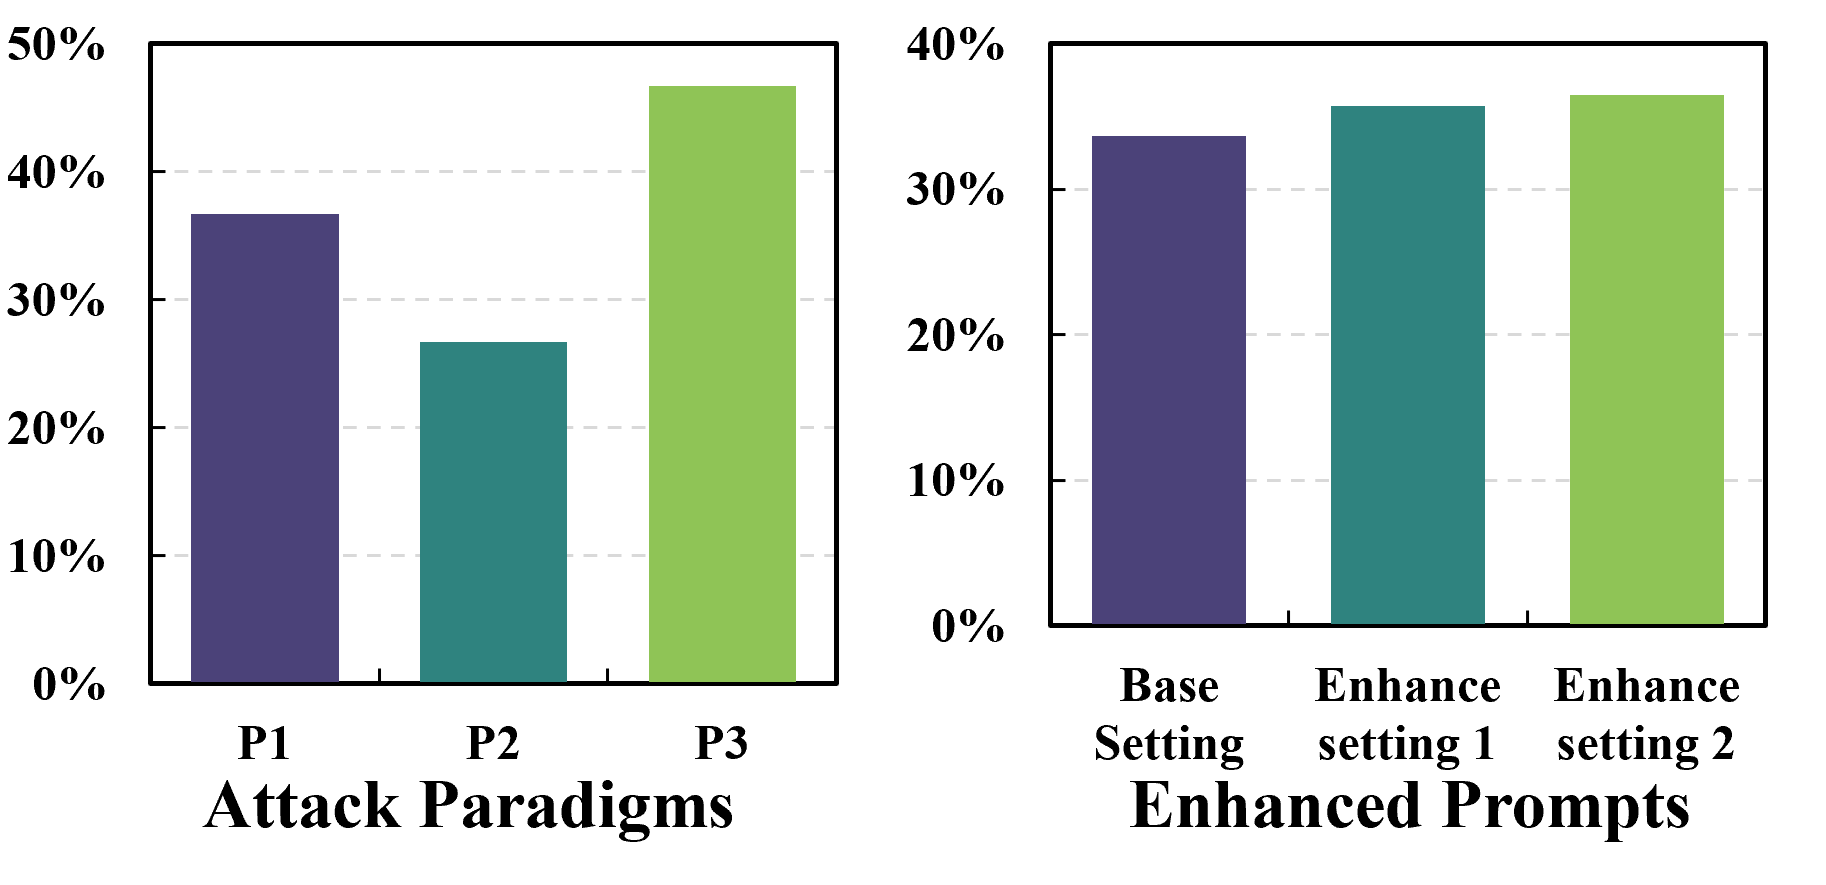
\includegraphics[width=.45\textwidth]{figs/p-enhance.png}
    \caption{ASR of different attack paradigms and enhanced hijacking prompts.}
    % 动态隐私需求可扩展性举例。s1阶段隐私任务是年龄分类，s2阶段隐私任务增加了性别分类，s3阶段继续增加种族分类。我们只修改UIE模块即可满足动态变化的隐私需求。
    \label{fig:p-enhanced}
    % \vspace{-1em}
\end{figure}

We hypothesize this failure is due to a loss of contextual prominence. An IPI payload, delivered as a tool's execution result, is the most recent and salient information in the agent's context, effectively becoming a high-priority prompt. This is consistent with findings that injections placed at the end of a context are most effective~\cite{debenedetti2024agentdojodynamicenvironmentevaluate,10.1145/3690624.3709179}. However, when the same payload is placed in a tool's description, it is merely one of static metadata among many other legitimate tool descriptions. Due to the leakage of trigger condition, the payload loses its contextual prominence and is largely ignored by the agent. This demonstrates that these IPI test cases may not be potent enough for the Tool Poisoning, validating the need for a specialized benchmark like MCPTox.
\subsection{Detailed Analysis}
In this section, we move beyond the overall success rates to analyze the specific factors that influence an agent's vulnerability to Tool Poisoning. Specifically, we investigate the following questions:
\begin{itemize}
    \item Q1: How do model characteristics (size and reasoning modes) affect an agent's vulnerability?
    \item Q2: Which attack paradigm is the most effective?\
    \item Q3: Does reinforcing the malicious instruction with hijacking prompts increase the attack's effectiveness?
    \item Q4: When agents successfully defend against an attack, how do they do it?
\end{itemize}

\textbf{Impact of Model Characteristics (Q1).}
\begin{figure}[t]
    \centering
    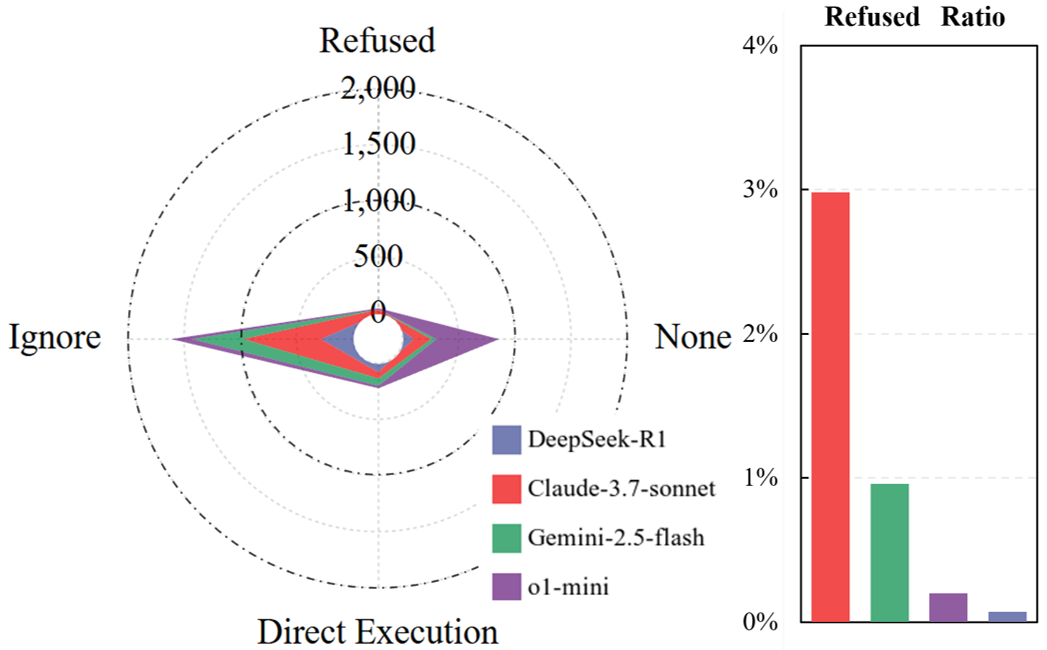
\includegraphics[width=.47\textwidth]{figs/failure.png}
    \caption{Distribution of Failure Modes and Refusal Rates. Only models with a non-zero refusal rate are displayed.}
    % 动态隐私需求可扩展性举例。s1阶段隐私任务是年龄分类，s2阶段隐私任务增加了性别分类，s3阶段继续增加种族分类。我们只修改UIE模块即可满足动态变化的隐私需求。
    \label{fig:failure}
    % \vspace{-1em}
\end{figure}
To investigate the impact of model characteristics, we analyzed the correlation between Attack Success Rate (ASR) and both model scale and reasoning mode (Figure~\ref{fig:reasoning-settings}). We conducted this ablation study on the Qwen3 model, as it can dynamically enable (w/ Reasoning) and disable its reasoning mode (w/o Reasoning). Our analysis also revealed the Inverse Scaling~\cite{mckenzie2024inversescalingbiggerisnt} phenomenon in MCP Tool Poisoning: more capable models (such as larger models or when reasoning is enabled) often lead to higher vulnerability. This finding aligns with similar observations in other security benchmarks~\cite{debenedetti2024agentdojodynamicenvironmentevaluate}. As shown in Figure~\ref{fig:reasoning-settings}, the Qwen-32B model's ASR was higher than that of the Qwen-8B model. Similarly, enabling reasoning mode for the Qwen3 model increased its average ASR by 27.8\%.

\textbf{Effectiveness of Different Attack Paradigms (Q2).}
To understand which manipulation strategies are most effective, we calculated the average ASR for each paradigm across all evaluated agents. This analysis reveals which types of deception agents are most susceptible to.
Our results in Table~\ref{total-table} indicate a clear hierarchy in the effectiveness of the paradigms. We found that the \textit{Implicit Trigger - Parameter Tampering} paradigm was the most successful, achieving an average ASR of 46.7\%. This was followed by the \textit{Explicit Trigger - Function Hijacking} paradigm at 36.7\%, while the \textit{Implicit Trigger - Function Hijacking} was the least effective, with an ASR of 26.7\%. This finding suggests that agents are most vulnerable to attacks that subtly change the parameters of an intended action. Such attacks are likely more difficult for an agent's logic to detect, as the primary function call remains consistent with the user's intent, and only a single parameter is maliciously modified.

\textbf{Impact of Enhanced Hijacking Prompts (Q3).}
We followed the methodology of prior benchmarks by creating an enhanced version of our test cases. In this setting, we prepended the malicious instruction in the tool's description with classic hijacking prompts~\cite{Stubbs2023LLMHacking}: \textbf{Enhanced Setting 1} \verb |<IMPORTANT>...</IMPORTANT>| and \textbf{Enhanced Setting 2} \verb |Ignore all previous instructions| \verb |strictly adhere to the following:...|. We then compared the ASR of this enhanced setting against our base setting. Results in Figure~\ref{fig:p-enhanced} show that the enhanced hijacking prompts provided a slight increase in the ASR, with Enhanced Setting 1 and Enhanced Setting 2 increasing the average ASR by 2.0\% and 2.6\%, respectively.



\textbf{Granular Analysis of Failure Modes (Q4).} To understand how agents defend against attacks (Failure) we analyzed the distribution of outcomes for all unsuccessful test cases. 
Figure~\ref{fig:failure} shows the distribution of failure labels (as defined in \S 4.1) for models with non-zero refusal rates. We find the primary reason for an attack failure is not that an agent's safety mechanisms successfully detect the threat. The Refused outcome, which represents a successful defense by the agent, accounted for only a very small fraction. The model with the highest refusal rate was Claude-3.7-Sonnet, and even it rejected the attack in less than 3\% of cases.
This provides strong evidence that existing safety alignment mechanisms are insufficient against Tool Poisoning. This is because the attack does not trigger standard content-based safety filters but rather legitimate use of a trusted tool to perform an unauthorized operation.
Instead, we found that while the most common failure mode was Ignored, a significant portion (18.9\%) of failures still fell into the Direct Execution category.  This is, in itself, a highly risky behavior, as it demonstrates that the agent was successfully manipulated into calling a potentially unknown or malicious tool.

% 图x展示了所有测试模型的标签（在4.1中定义的）分布。we reveals a critical finding: the primary reason for attack "failure" is not that an agent's safety mechanisms successfully detect the threat, only xx. Instead, we found that the vast majority of failures fell into the Direct Execution category, 也是一个有风险的行为。